\documentclass[plainsections, 32pt]{sciposter}

\usepackage[brazil]{babel}		% Idioma do documento
\usepackage{xcolor}			    % Controle das cores
\usepackage[T1]{fontenc}		% Selecao de codigos de fonte.
\usepackage{graphicx}			% Inclusão de gráficos
\usepackage[utf8]{inputenc}		% Codificacao do documento (conversão automática dos acentos)
\usepackage{wallpaper}
\usepackage{wrapfig}
\usepackage{amsfonts,amssymb,amsmath,amsthm}
\usepackage{multicol}
\usepackage{anyfontsize}
\usepackage{braket}
\usepackage{anyfontsize}

\providecommand{\U}[1]{\protect\rule{.1in}{.1in}}
%EndMSIPreambleData
\setcounter{tocdepth}{4}

%opening
\definecolor{amarelo}{HTML}{FFCC00}
\definecolor{verde}{HTML}{006600}
\renewcommand{\papertype}{custom}
\setlength{\paperwidth}{90cm}
\setlength{\paperheight}{100cm}
\renewcommand{\setpspagesize}{
\ifthenelse{\equal{\orientation}{portrait}}{
\special{papersize=90cm,100cm}
}{\special{papersize=90cm,100cm}}}
\setlength{\topmargin}{0in}
\setlength{\headheight}{0in}
\setlength{\headsep}{0in}
\setlength{\textheight}{84cm}
\setlength{\textwidth}{75.5cm}
\setlength{\oddsidemargin}{2.4cm}
\setlength{\evensidemargin}{0cm}
\setlength{\parindent}{0.25in}
\setlength{\parskip}{0.25in}
\setlength{\pdfpagewidth}{90cm}
\setlength{\pdfpageheight}{100cm}
\newcommand\BackgroundPic{
\put(-82,65){
\parbox[b][\paperheight]{\paperwidth}{
\vfill
\centering

\includegraphics[width=\paperwidth,height=\paperheight,
keepaspectratio]{poster-xi-sic-2.jpg}
\vfill
}}}
\setlength{\columnseprule}{0pt}

\renewcommand{\titlesize}{\fontsize{68}{40}\selectfont }
\newcommand{\largo}{\fontsize{36}{40}\selectfont }
\makeatletter



% Redefine a função section
\renewcommand\section{\@startsection {section}{1}{\z@}{-1ex \@plus -0.5ex \@minus -.1ex}{0.8ex \@plus.1ex}{\largo\bfseries\fontsize{28}{26}\selectfont}}

\makeatother
\vspace{-3cm}

\def\thesection{}
%%% Título %%%
\title{\vspace{-3.3cm} \hspace{-28cm}\textcolor{amarelo}{\parbox{0.9\textwidth}{Mapeamento Clássico-Quântico: Um Estudo do Modelo de Ising em Duas Dimensões}}}
%%%
\usepackage{parskip}
\begin{document}

\AddToShipoutPicture{\BackgroundPic}
\makeatletter
\AddToShipoutPicture{%
            \setlength{\@tempdimb}{.5\paperwidth}%
            \setlength{\@tempdimc}{.5\paperheight}%
            \setlength{\unitlength}{1pt}%
            \put(\strip@pt\@tempdimb,\strip@pt\@tempdimc){%
                    }%
}
\makeatother
\maketitle
\mbox{}\vspace{0cm}

\begin{center}
\textbf{{\large Alex Enrique Crispim}}\\
Centro de Ciências Naturais e Humanas - UFABC\\
Av. dos Estados, 5001, Santo André, SP\\
\textit{alex.enrique@ufabc.edu.br}
\end{center}

\vspace{1cm}
\begin{multicols}{2}
\paragraph{Resumo:} Neste trabalho, estudou-se a técnica do \textit{mapeamento clássico-quântico}, aplicada ao Modelo de Ising. O objetivo final do projeto era extrair informações da versão quântica do modelo unidimensional usando este formalismo. Isso se deu calculando computacionalmente observávais quânticos, utilizando o modelo clássico em duas dimensões.

\textbf{Palavras-chave:} Modelo de Ising, Mecânica Quântica, Mecânica Estatística, Transição Quântica de Fase, Sistemas Quânticos de Muitos Corpos. Sistemas Fortemente Correlacionados.

\section*{Introdução}
\vspace{-3mm}
De forma geral, acredita-se, que a função de partição de um modelo quântico de dimensão $D$ pode ser mapeada exatamente na função de partição de um modelo clássico de dimensão $D+1$.
Este mapeamento tem sido fundamental para o estudo de teorias fortemente correlacionadas. Em especial, a aplicação deste formalismo ao Modelo de Ising leva à formulação de um modelo quântico de fundamental importância para o estudo de transições quânticas de fase e o entendimento de transições de fase de segunda ordem.

\section*{O Modelo de Ising}
\vspace{-3mm}
O Modelo Clássico de Ising em duas dimensões corresponde a uma rede de variáveis clássicas $\sigma_i$ que assumem valores $\pm 1$ (spin para cima ou para baixo). Essas se encontram arranjadas em uma rede bidimensional, normalmente quadrada (Figura 1). O modelo apresenta uma transição de fase à temperatura $T_c$ finita e tem a Hamiltoniana $H_{Ising}$, apresentadas em (1) (Ising, 1925; Onsager, 1944).
\begin{equation}
  H_{Ising} = - J \sum_{\braket{i, j}} \sigma_i \sigma_j,
  \qquad \frac{J}{k_b T_c} = \frac{\log(1+\sqrt{2})}{2}
\end{equation}
com $\braket{i, j}$ representando os $j$ primeiros vizinhos de $i$ e $k_b$ sendo a constante de Boltzmann.

\begin{figure}
  \center
  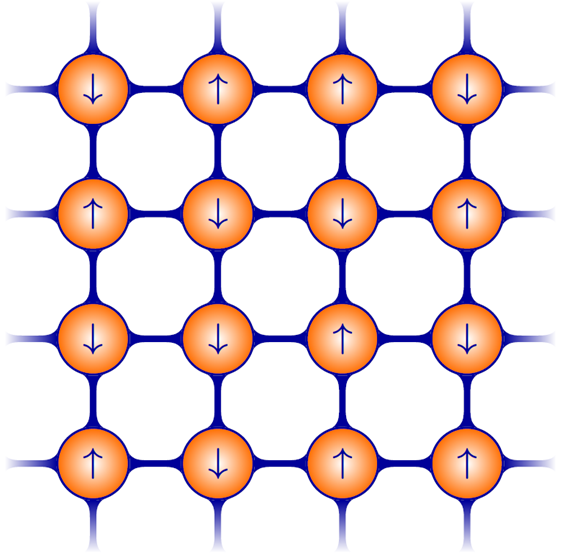
\includegraphics[scale = .9]{lattice.png}
  \caption{Exemplo de uma rede quadrada de spins. Fonte: https://quantumoptics.at/}
\end{figure}

\vspace{-15mm}
A função de partição desta Hamiltoniana clássica, pode ser mapeada exatamente na função de partição da \textit{Hamiltoniana Quântica de Ising Unidimensional} (Figura 2), $\hat{H}_\Delta$, da forma
\begin{equation}
  \hat{H}_{\Delta} = -J\sum_i \hat{\sigma}_{i}^z \hat{\sigma}_{i+1}^z + \Delta \hat{\sigma}_i^x.
\end{equation}
Para este modelo quântico, a transição de fase ocorre quando $\Delta = 1$.

\begin{figure}
  \center
  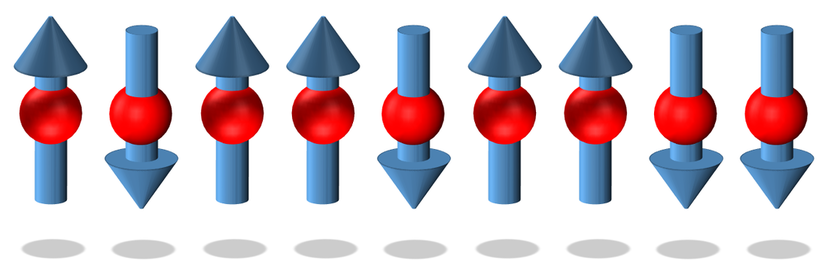
\includegraphics[scale = .45]{chain.png}
  \caption{Cadeia de spins quânticos unidimensional. Fonte: (Veltman, 2016)}
\end{figure}

\vspace{-15mm}
Utilizando a técnica do mapeamento clássico-quântico, é possível estudar este modelo quântico na transição de fase, por meio do modelo clássico bidimensional. As vantagens se dão em termos de menor complexidade computacional e no uso de uma teoria clássica (mecânica estatística clássica), costumeiramente mais simples de se trabalhar e mais intuitiva.

\section*{Desigualdades de Bell e Correlações Quânticas}
\vspace{-3mm}
Na década de 60, John Bell derivou uma desigualdade acerca do valor esperado de variáveis aleatórias $Q, R, S, T$ que assumem valores $\pm 1$, sob as hipóteses do paradoxo EPR (paradoxo de Einstein-Podolsky-Rosen) (Einstein \textit{et al}, 1935; Bell, 1964). A desigualdade afirma que o valor esperado da quantidade $QS + RS + RT - QT$ é tal que
\begin{equation}
  \braket{QS + RS + RT - QT} \leq 2.
\end{equation}
O interesse nesta desigualdade foi a verificação de que a mesma se faz incompatível com experimentos, mostrando que a natureza comporta-se conforme a Mecânica Quântica prevê.

Em especial, para o estados emaranhados
\begin{equation*}
  \ket{\Psi^-} = \frac{\ket{\uparrow \downarrow} - \ket{\downarrow \uparrow}}{\sqrt{2}},
  \qquad
  \ket{\Phi^+} = \frac{\ket{\uparrow \uparrow} + \ket{\downarrow \downarrow}}{\sqrt{2}}
\end{equation*}
com os observáveis
\begin{equation*}
  Q = Q^\prime = \sigma_1^z, \quad R = R^\prime = \sigma_1^x, \quad S = -S^\prime = \frac{-\sigma_2^z - \sigma_2^x}{\sqrt{2}}, \quad T = -T^\prime =  \frac{\sigma_2^z - \sigma_2^x}{\sqrt{2}}
\end{equation*}
tem-se os valores esperados
\begin{equation}
  \braket{\Psi^-|(QS + RS + RT - QT)|\Psi^-} = \braket{\Phi^+|(Q^\prime S^\prime + R^\prime S^\prime + R^\prime T^\prime - Q^\prime T^\prime)|\Phi^+} = 2\sqrt{2}  > 2.
\end{equation}

Para este trabalho, avaliou-se os valores esperados em (4) para primeiros vizinhos de uma cadeia quântica de Ising. Se, para alguma temperatura, o sistema se encontrasse nos estados $\ket{\Psi^-}$ ou $\ket{\Phi^+}$, a desigualdade de Bell deveria ser violada.

\section*{Resultados}
A Figura 3 mostra o gráfico em função da temperatura (unidades arbitrárias, definindo $k_b = 1$). A transição de fase ocorre para a temperatura aproximada de $2,27$. Dos gráficos, é possível perceber um aumento das correlações próximo à transição de fase. Além disso, nota-se que a desigualdade de Bell é violada apenas para o estado $\ket{\Phi^+}$, como esperado de um sistema ferromagnético, pois nesse, os spins tendem a serem encontrados alinhados.
\vspace{2mm}
\begin{figure}
  \center
  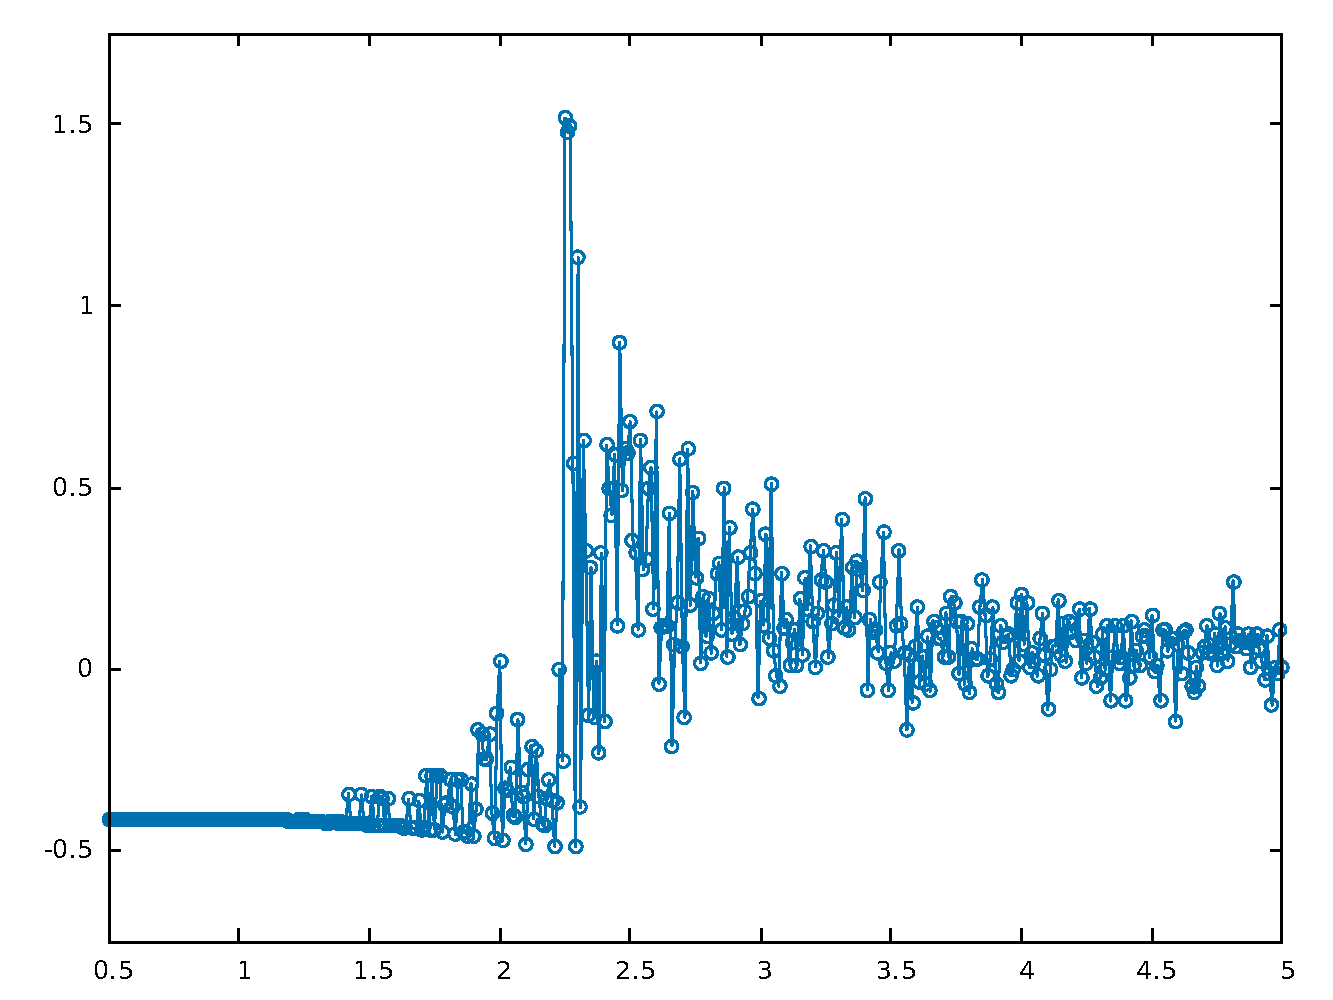
\includegraphics[scale = .7]{result3.pdf}
  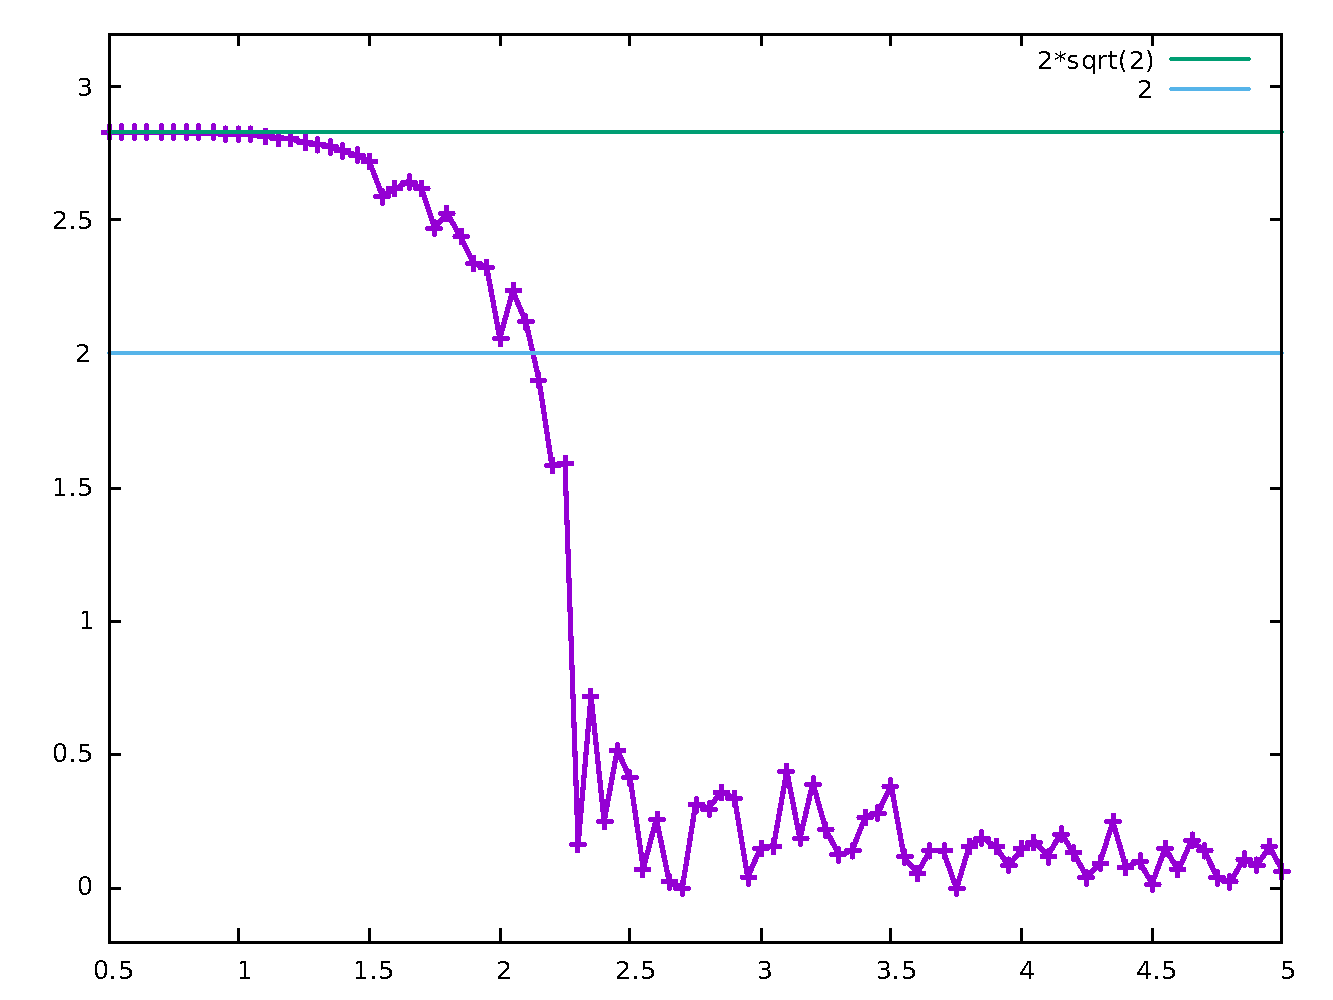
\includegraphics[scale = .7]{bell.pdf}
  \caption{Valores esperados $\braket{\Psi^-|(QS + RS + RT - QT)|\Psi^-} $ (gráfico em azul) e $ \braket{\Phi^+|(Q^\prime S^\prime + R^\prime S^\prime + R^\prime T^\prime - Q^\prime T^\prime)|\Phi^+}$ (gráfico em roxo) em função da temperatura (unidades dadas definindo-se a constante de Boltzmann igual a 1).}
\end{figure}


\vspace{-5mm}

\section*{Conclusão}
\vspace{-2mm}
Este trabalho mostrou que na transição de fase do Modelo Quântico de Ising unidimensional as correlações entre os spins aumentam. Por meio do estudo de dois funcionais de Bell, mostrou-se que não ocorre a formação dos estados $\ket{\Psi^-}$, na média temporal, e que os primeiros vizinhos encontram-se emaranhados no estado $\ket{\Phi^+}$ para $T < T_C$. Por fim, o resultado obtido mostra a violação da Desigualdade de Bell, verificando que a cadeia de spins se comporta como previsto pela Mecânica Quântica.


\section*{Referências}
Ising, E. (1925). Beitrag zur Theorie des Ferromagnetismus. Zeitschrift für Physik, 31:253–258.

Onsager, L. (1944). ``Discussion'', Nuovo Cimento (suppl.) 6 , 261.

Einstein, A.; Podolsky, B.; Rosen, N. (1935). ``Can Quantum-Mechanical Description of Physical Reality Be Considered Complete?''. Physical Review. 47 (10): 777–780.

Bell, John. (1964). ``On the Einstein Podolsky Rosen Paradox''. Physics. 1 (3): 195–200.

Veltman, T. (2016). Heisenberg Spin Chains with
Boundaries and Quantum Groups. Master Thesis, University of Amsterdam.

\section*{Agradecimentos}
Agradeço ao meu orientador, professor Eduardo Peres Novais de Sá, por me apresentar aos vários temas estudados durante este projeto e pelo acompanhamento ao longo da minha jornada acadêmica na UFABC, estando sempre disposto a ajudar de alguma forma.

Agradeço de forma geral a cada uma das pessoas que me ajudaram das mais diversas formas, ao longo do projeto e na jornada até o presente.

Em especial, reservo um agradecimento ao Programa de Iniciação Científica PIBIC do CNPq, o qual financiou este trabalho.

\clearpage % remover ao final

\end{multicols}

\end{document}
